\section{The A\lowercase{tomic}O\lowercase{rchid} Game}\label{sec:atomicorchid}
\noindent In this section we describe the AtomicOrchid game used to embed the planning agent in order to trial mixed-initiative coordination.
We adopt a serious mixed-reality games approach to counteract the limitations of computational simulations \cite{Fischer:etal:2012}. For example, Simonovic highlights that simulations may rely on unrealistic geographical topography, and most importantly, may not account for ``human psychosocial characteristics and individual movement, and (...) learning ability'' \cite{simonovic:2009}. The impact of emotional and physical responses likely in a disaster, such as stress, fear, exertion or panic remains understudied in approaches that rely purely on computational simulation \cite{drury:etal:2009}. In contrast, our approach creates a realistic setting in the sense that participants experience physical exertion and stress through bodily activity and time pressure, mirroring aspects of a real disaster setting \cite{paho:2001}. This, in turn, provides greater confidence in the efficacy of behavioural observations regarding team coordination supported by a planning agent.

In more detail, AtomicOrchid is a location-based mobile game based on the fictitious scenario described in Section \ref{sec:scenario}. First responders are assigned a specific type: medic, fire-fighter, soldier, or transporter. Their mission is to evacuate all four types of targets: victim (requires medic and fire-fighter), animal (requires medic and transporter), fuel (requires soldier and fire-fighter), or other resource (requires soldier and transporter).  The first responders are supported by (at least) one person $H$ in a centrally located HQ room, and the planning agent $PA$ that sends the next task (as described in the previous section) to the team of first responders. In what follows, we present the player interfaces used, the interactions with the planning agent, and the modelling of the radiation cloud in the game. A video of the operation of AtomicOrchid can be viewed at: \url{http://bit.ly/1ebNYty}.

\subsection{Player Interfaces}
\noindent First responders are equipped with a `mobile responder tool' providing sensing and awareness capabilities in three tabs (geiger cou\-nter, map, messaging and tasks; see Figure \ref{fig:ui}). The first tab shows a reading of radioactivity, player health level (based on exposure), and a GPS-enabled map of the game area to locate fellow responders, the targets to be rescued and the drop off zones for the targets. The second tab provides a broadcast messaging interface to communicate with fellow first responders and the commander $H$. The third tab shows the team and task allocation dynamically provided by the agent $PA$ that can be accepted or rejected. Notifications are used to alert both to new messages and task allocations.

\begin{figure}[htbp]
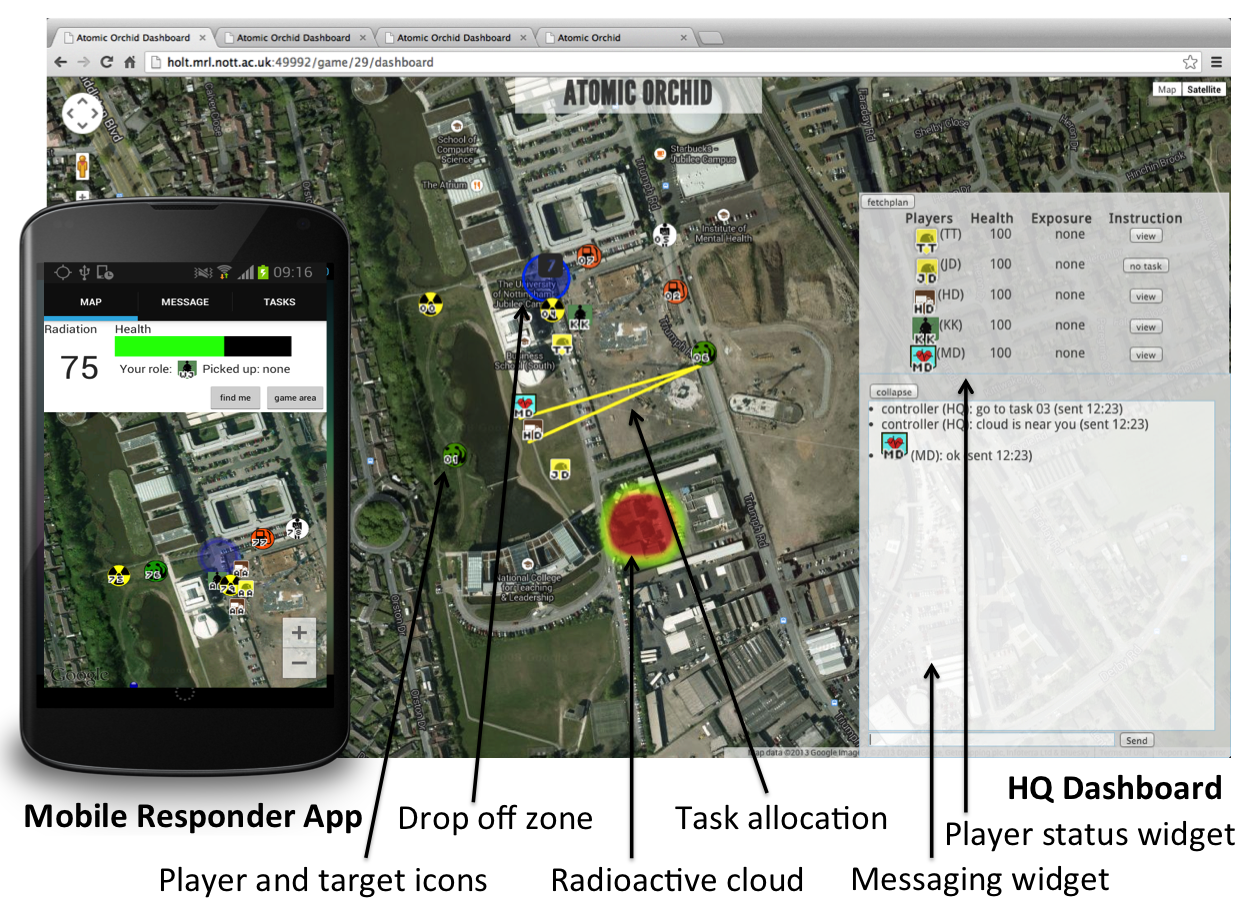
\includegraphics[width=\columnwidth]{UI.png}
\caption{Mobile first responder and HQ interfaces.}\vspace{-3mm}
\label{fig:ui}
\end{figure}

<<<<<<< HEAD
$H$ has at her disposal an `HQ dashboard' that provides an over\-view of the game area, including real-time information of the players' locations (see Figure \ref{fig:ui}). The dashboard provides a broadcast messaging widget, and a player status widget so that the responders' exposure and health levels can be monitored. $H$ can further monitor the  current team and task allocations to individual responders by $PA$ (by clicking on a button). Crucially, only $H$ and $PA$ have a view of the radioactive cloud, graphically depicted as a heatmap (`Hotter'  (red) zones correspond to higher levels of radiation). \\

\noindent Importantly, the cloud is only known by the HQ, not field responders. In real world disaster operations, it is likely that HQ and field teams have different sources of information, and they have to communicate with available communication channels (e.g. text, messages ) . The design decision is aimed to simulate this characteristic of DR operation. 
=======
$H$ has at her disposal an `HQ dashboard' that provides an over\-view of the game area, including real-time information of the players' locations (see Figure \ref{fig:ui}). The dashboard provides a broadcast messaging widget, and a player status widget so that the responders' exposure and health levels can be monitored. $H$ can further monitor the  current team and task allocations to individual responders by $PA$ (by clicking on a button). The radioactive cloud is graphically depicted as a heatmap (`Hotter'  (red) zones correspond to higher levels of radiation). Crucially, only  $H$ can 'see' the entire cloud, while field responders are restricted to seeing a reading for their current location on their Geiger counters --- this is a deliberate design choice to require frequent communication between HQ and field responders. 
>>>>>>> 2596b2bc39dc5789e3bd39ca2241aa3bd2a26abf

\subsection{System Architecture}
\noindent AtomicOrchid is based on the open-sourced geo-fencing game MapAttack\footnote{\url{http://mapattack.org}.} that has been iteratively developed for a responsive, (relatively) scalable experience.  The location-based game is underpinned by client-server architecture, that relies on real-time data streaming between client and server. Client-side requests for less dynamic content use HTTP. Frequent events (e.g., location updates and radiation exposure) are streamed to clients to avoid the overhead of HTTP. In this way, first responders are kept informed in near real-time. Finally,  to build the mobile app, we adapted the existing MapAttack Android app.

%The platform is built using the geoloqi platform, Sinatra for Ruby, and state-of-the-art web technologies such as socket.io, node.js and the Google Maps API. 

\subsection{Integrating the Planning Agent}
\noindent The planning agent $PA$ takes the game status (i.e., positions of players, known status of the cloud, and messages received from players) as input and produces a plan for each responder  for the current state. $PA$ is deployed on a separate server. The AtomicOrchid server requests a plan from the agent via a stateless HTTP interface by transmitting the game status in JSON format. Polling (and thus re-planning) is triggered by two types of game events:
\begin{itemize}
\item \textit{Completion of task}. On successful rescue of a target, a new plan (i.e., allocation of tasks to each responder) is requested from the agent.
\item \textit{Explicit reject}. On rejection of a task allocation by any of the allocated first responders, a new plan is requested.  More importantly, the rejected allocation is, in turn, used as a constraint within the optimisation run by the planner agent (as described in Section \ref{sec:adaptive}). For example, if two responders, one medic and one soldier, were allocated a task and the medic rejected it, the planning agent would rerun the optimisation algorithm with the constraint that this medic should not be allocated this task. If another medic is free (and accepts) the soldier and this medic can go ahead and complete the task. Otherwise, a new plan is created for the soldier.
\end{itemize} 

\todo{GOPAL: add architecture diagram showing how agent and human interact}

%\subsection{Interacting with planning agent}
%There can interact directly with field players through a task tab (Figure xx) and agent plans are also visible to HQ's dashboard interface.
Once a plan is received from $PA$, the AtomicOrchid game engine splits the plan for a given team into individual task allocations for each player and sends them to their mobile responder app. The app presents the task allocation in the task tab, detailing: i) the responder to team up with, ii) the allocated target (using target id), and iii) approximate direction of the target (e.g., north, east).  Once a player accepts a task, an acknowledgement is sent to their teammate, while rejecting a task triggers a new assignment from $PA$. 

%Furthermore, $H$ is provided with a visualisation of task allocations for each player on demand (by button press), to help monitor the task allocation computed by the agent.


\subsection{Radiation Cloud Modelling}\label{sec:radiation}
\noindent The radiation cloud is assumed to be monitored using a number of sensors on the ground (within the disaster space) that collect readings of the radiation cloud intensity and wind velocity every minute of the game. These sensors can be at fixed locations or held by mobile agents.  The radiation cloud diffusion process is modelled in a standard way by a nonlinear Markov field stochastic differential equation,  
\begin{eqnarray*}
\frac{D \text{Rad}({\bf z}, \tau)}{D \tau}=\kappa \triangledown^2 \text{Rad}({\bf z},\tau)-\text{Rad}({\bf z},\tau)\triangledown \cdot {\bf w}({\bf z},\tau)+\sigma({\bf z},\tau)
\end{eqnarray*}
where $D$ is the material derivative, $\text{Rad}({\bf z},\tau)$ is the radiation cloud intensity at location ${\bf z}$ at time $\tau$, $\kappa$ is a fixed diffusion coefficient and $\sigma$ is the radiation source(s) emission rate. The diffusion equation is solved on a regular grid defined across the environment with grid coordinates $G$ (as defined in Section \ref{sec:model}).  Furthermore, the grid is solved at discrete time instances $\tau$.  The cloud is driven by wind forces which vary both spatially and temporally.  These forces induce anisotropy into the cloud diffusion process which is proportional to the wind velocity, ${\bf w}({\bf z},\tau)$.  The wind velocity is drawn from two independent Gaussian processes (GP), one GP for each Cartesian coordinate axis, $w_i({\bf z},\tau)$, of ${\bf w}({\bf z},\tau)$.  The GP captures both the spatial distribution of the wind velocity and the dynamic process resulting from shifting wind patterns such as short term gusts and longer term variations. 

% In our simulation, each spatial wind velocity component is modelled by a squared-exponential GP covariance function, $K$, with fixed input and output scales (although any covariance function can be substituted). Furthermore, as wind conditions may change over time we introduce a temporal correlation coefficient, $\rho$, to the covariance function.  Thus, for a single component, $w_i$, of ${\bf w}$, defined over grid $G$ at times $\tau$ and $\tau^\prime$, the wind process covariance function is, $\text{Cov}(w_i(G,\tau),w_i(G,\tau^\prime))=\rho(\tau,\tau^\prime) K(G,G)$.  We note that, when $\rho=1$ the wind velocities are time invariant (although spatially variant).  Values of $\rho<1$ model wind conditions that change over time.

Using the above model, we are able to create a moving radiation cloud, thus posing a real challenge both for the HQ (agent and commander) and the responders on the ground, as predictions they can make of where the cloud will move to will be prone to uncertainty both to the simulated wind speed and direction. 


%(\textbf{Steve: in the platform we take the `real' values from the diffusion process i believe. Does the above capture this? We will say that we will add the features you mention below to a future version of the platform where we aim to do both situational awareness and rescue. Add a sentence above to conclude where we took the values from and the process takes into account the  location of radiation source. Also, your notation clashes with the notations in the scenario and Feng's algorithm - please try to align.}
%The cloud intensity and wind velocity are measured by {\it monitor agents} equipped with geiger-counters and anemometers.  These agents are directed to take measurements with greatest information gain in the radiation cloud intensity.  The measurements are folded into the EKF and this refines estimates of the radiation cloud across the grid.  Figure~\ref{radiation_screen_shots} shows example cloud simulations for slow varying (i.e. $\rho=0.99$) and gusty (i.e. $\rho=0.90$) wind conditions.  Figure~\ref{radiation_screen_shots}(a) shows slow varying wind conditions in which case the radiation cloud can be interpolated accurately using sparse sensor measurements and the LFM model.  Alternatively, during gusty conditions the radiation cloud model is more uncertain far from the locations where recent measurements have been taken, as shown in Figure~\ref{radiation_screen_shots}(b).
%
%\begin{figure}[ht] \begin{center}
%    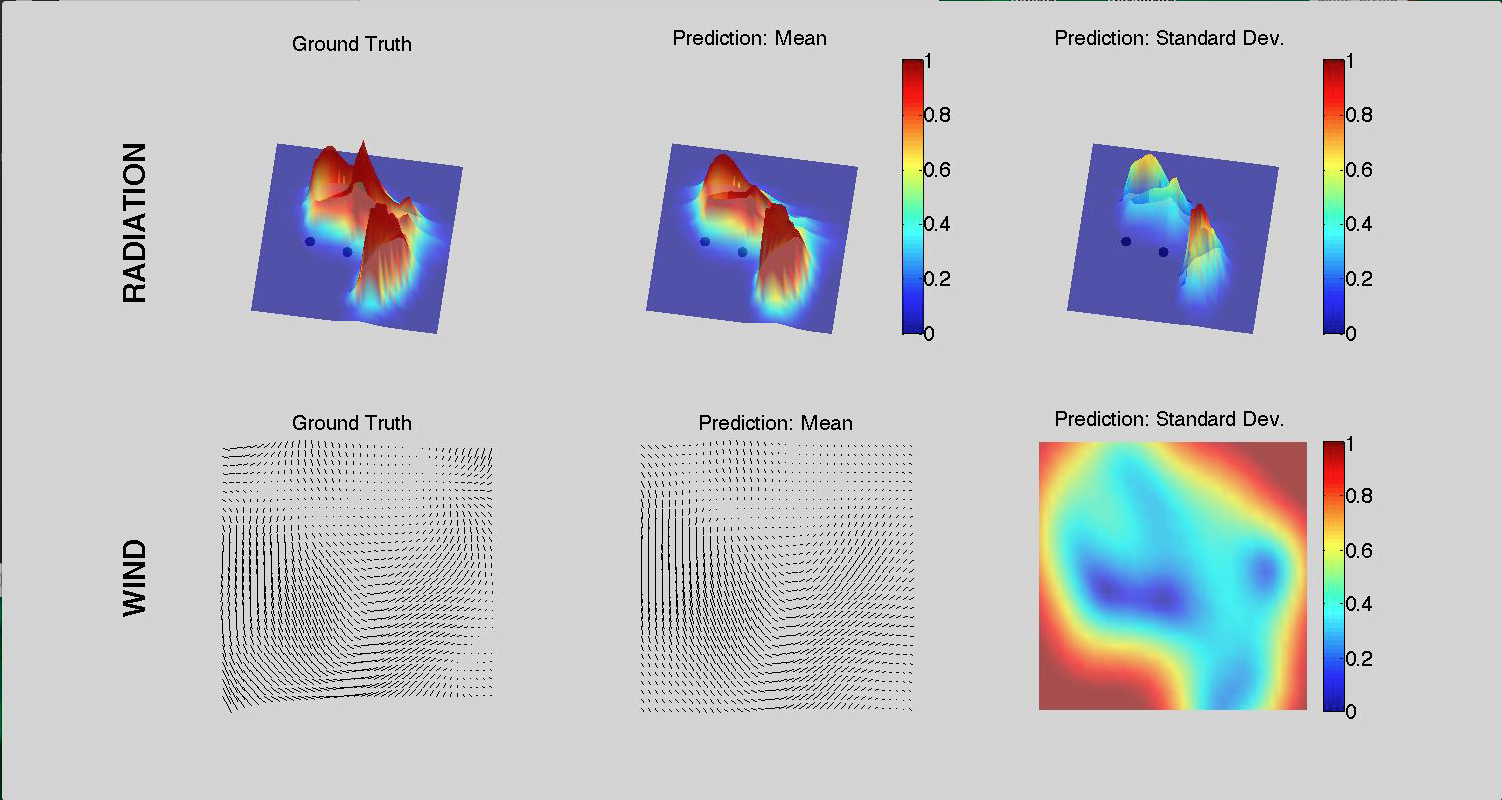
\includegraphics[width=0.45\textwidth]{figures/radiation_ss_calm.png}\\
%    (a) Slowly varying wind conditions\\ \ \\
%    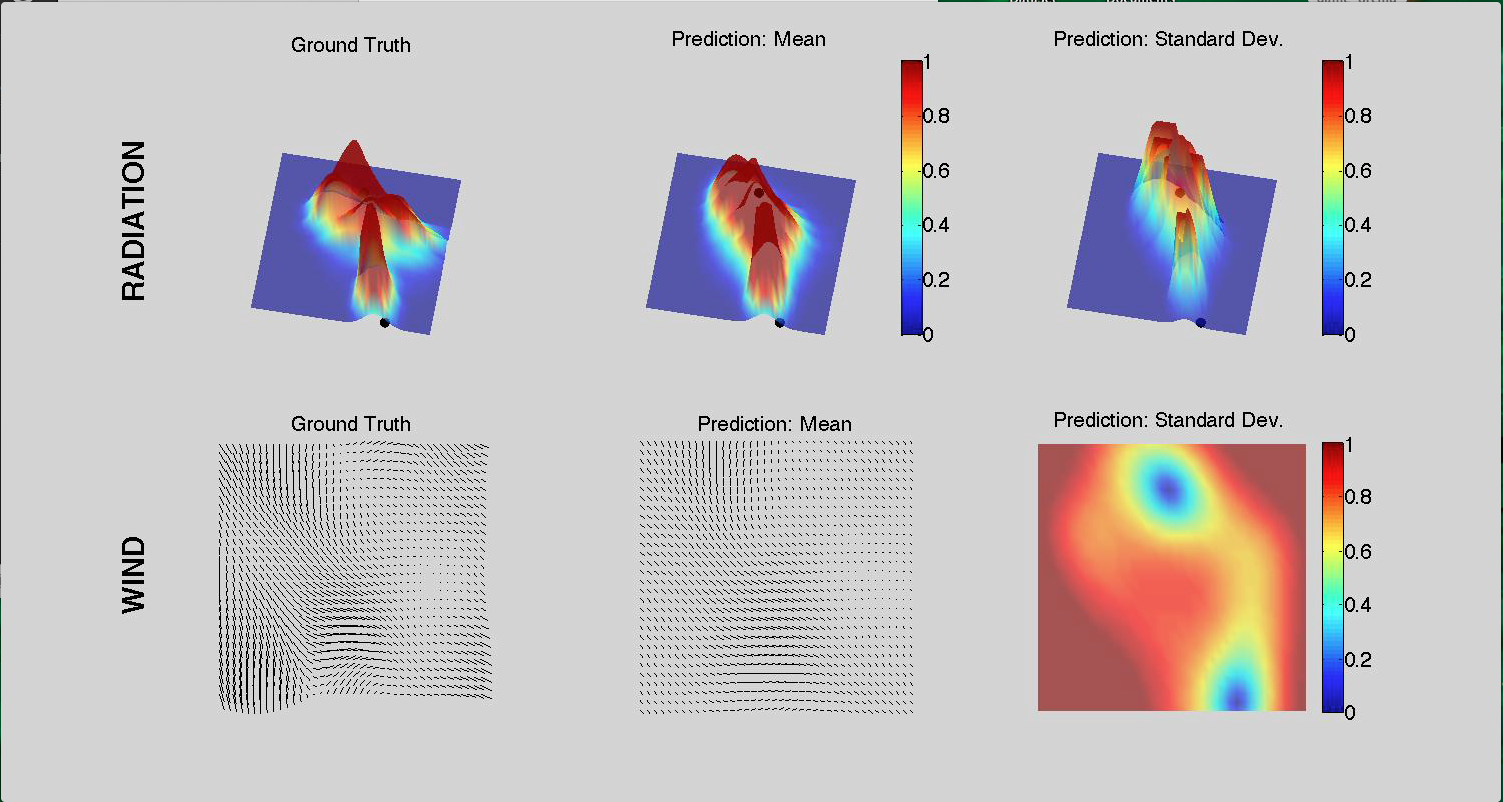
\includegraphics[width=0.45\textwidth]{figures/radiation_ss_gust.png}\\
%    (b) Gusty wind conditions 
%\caption{\label{radiation_screen_shots} Radiation and wind simulation ground truth and EKF estimates obtained using measurements from monitor agents (black dots).  Left most panes are ground truth radiation and wind conditions, the middle panes are corresponding estimates and right most panes are state uncertainties:  (a) Invariant and (b) gusty wind conditions.}
%\end{center}
%\end{figure}

\section{Field Trialling AtomicOrchid}\label{sec:evaluation}
\noindent We ran three sessions of AtomicOrchid with participants recruited from the local university to trial mixed-initiative coordination in a disaster response scenario. The following sections describe the participants, procedure, session configuration and methods used to collect and analyse quantitative and qualitative data.

\subsection{Participants and Procedure}
%\noindent We do not attempt to run tens or hundreds of trials to generate statistically significant results. Rather, we focus on running enough trials to gain an insight into how participants perceive and interact with our planning agent. This approach is advocated in  \cite[p. 1663]{Brown:2011:WCO:1978942.1979185}, in which participants in field trials are experts on their own activity.  These experts attempt to predict what might happen with a particular technology, to develop insights based on their use of it.  In particular,  \cite{Brown:2011:WCO:1978942.1979185} point to the fact that running multiple trials (in an attempt to obtain statistical significant results)  has no relationship to  insightfulness.  Crucially, they suggest that  participants can be seen as investigators themselves in the  trial, with a move to acknowledging that it is through  participants' own insights that the power of the trials can be focused.
%


%\noindent As argued by \cite[p. 1663]{Brown:2011:WCO:1978942.1979185}, participants in field trials are used as experts on their own activity, attempting to predict what might happen with  a particular technology, to develop insight based on their  use.  In particular, they point to the fact that running multiple trials (in an attempt to obtain statistical significant results)  has no relationship to  insightfulness.  Crucially, they suggest that  participants can be seen as investigators themselves in the  trial, with a move to acknowledging that it is through  participants� own insights that the power of the trials can be focused. Hence, in line with this argument, we do not attempt to run tens or hundreds of trials to generate statistically significant results. Rather, we focus on running enough trials to gain an insight into how participants perceive and interact with our planning agent.
%

\noindent Our approach to field trials is strongly influenced by \cite[p. 1663]{Brown:2011} who state that ``participants in field trials are used as experts on their own activity, attempting to predict what might happen with a particular technology, to develop insight based on their  use".  In particular, they point to the fact that running multiple trials (in an attempt to obtain statistically significant results)  has no relationship to  insightfulness.  Crucially, they suggest that  participants can be seen as investigators themselves in the trial. Hence, in line with this argument, we do not attempt to run tens or hundreds of trials on many different scenarios to generate statistically significant results. Rather, we focus on running enough trials to gain an insight into how participants \emph{perceive} and \emph{interact} with our planning agent.

Hence, a total of 24 participants (17 males and 7 females) were recruited through posters and emails, and reimbursed with \pounds 15  for 1.5-2 hours of study. The majority were students. The procedure consisted of 30 minutes of game play, and about 1 hour in total of pre-game briefing, consent forms,  a short training session, and a post-game group discussion. The participants were told that their goal was to save as many targets as possible (out of a total of 20) before being engulfed by the `radioactive cloud'. Observations in the trial (such as running and screaming players) showed that this game mechanic put participants under the kind of stress that incites a real visceral response, supporting the objective of our mixed-reality game approach (see section \ref{sec:simulationvgames}).

%Upon arrival in the HQ (set up in a meeting room at the local university), participants were briefed and asked to consent to participate. They were presented with a demographic questionnaire to record gender, occupation, experience of using smartphones and level of map navigation skills.

At the end of the briefing, in which mission objectives and rules were outlined, FR types were randomly assigned to all participants (fire-fighter, medic, transporter, soldier). The HQ was staffed by a different member of the research team in each session in order to mimic an experienced $H$, while avoiding the same person running the HQ every time.  Moreover, FRs were provided with a smartphone and $H$ with a laptop. The team was given 5 minutes to discuss a common game strategy. 

FRs were then accompanied to the starting point within the designated game area, about 1 minute walk from headquarters. Once FRs were ready to start, $H$ sent a `game start' message. After 30 minutes of game play the FRs returned to the HQ where a group interview was conducted, before participants were debriefed and dismissed.

\subsection{Game Sessions}
\noindent We ran one session without $PA$, and two sessions with $PA$ to be able to compare team performance in the two versions. Each session involved \emph{different} sets of FRs (8 each). Thus,  players were unique to a session to avoid learning effects between sessions. While we cannot rule out learning effects \textit{within} sessions, we accept this as an integral part of working with humans in the real world. 

We also ran a pilot study for each condition to fine tune game configuration. The 8 FRs in each session were randomly allocated a role so that the whole team had two of each of the four types of FRs. The terrain of the 400x400 metre  game area includes grassland, a lake, buildings, roads,  footpaths and lawns. There were two  drop-off zones and 16 targets in each session. There were four targets for each of the four target types. The target locations, pattern of cloud movement and expansion were kept constant for all game sessions. The pilot study showed that this was a challenging, yet not too overwhelming configuration of game area size, and number of targets to collect in a 30 min game session. 

\subsection{Data Collection and Analysis}
\noindent We collected more than 20 hours of video of participants at the HQ, and participants on the ground (using multiple cameras to follow multiple teams at the same time). Video recordings of field action were catalogued to identify sequences (episodes) of interest through identification of key decision points in teaming and task allocation. Interesting distinct units of interaction were transcribed and triangulated with log files of relevant game activity for qualitative interaction analysis, presented in detail elsewhere \cite{Jiang2014}. For the purposes of the analysis presented here, we analysed the video data to classify how the agent task allocations were handled by humans. 

In addition, we developed a log file replay tool to triangulate video recordings of game action with the timestamped system logs that contain a complete record of the game play, including FRs' GPS location, their health status and radioactive exposure, messages, cloud location, locations of target objects and task status.

%Video recordings of field action were catalogued to identify sequences (episodes) of interest (cf. Heath et al., 2010). Key decision points in teaming and task allocation served to index the episodes. Interesting distinct units of interaction were transcribed and triangulated with log files of relevant game activity for deeper analysis. Due to space constraints we can only  present one fragment in this paper to illustrate how human-agent collaboration typically unfolded (TODO).

In this paper, we present an analysis of both $PA$'s task allocations and the messages sent between FRs and $H$ to support coordination in order to assess how humans interact with each other and with $PA$. In particular, we use speech-act theory \cite{searle:1975} to classify the messages composed by humans. We focus on the most relevant types of acts in this paper (which are also the most frequently used in AtomicOrchid):

\begin{itemize}
\item Assertives: \textit{speech acts that commit a speaker to the truth of the expressed proposition}; these were a common category as they include messages that contain situational information (e.g., You are next to the radiation cloud or the task is North of your current position).
\item Directives: \textit{speech acts that are meant to cause the hearer to take a particular action}; requests, commands and advice, including task and team allocation messages (e.g., X go to task 1, Y go with X).
\end{itemize}

\subsection{Results}
\noindent  The participants were seen to engage engage with the game scenario, showing signs of stress when targets could not be saved, and at times, running to save targets before these were covered by the radioactive cloud. This confirmed that the fun factor of the game helped to incentivise the participants to optimise their task allocation plans. 

Overall, 8 targets were rescued in the non-agent condition (Session A), and respectively 12 targets (Session B) and 11 targets (Session C) were rescued in the agent condition. Teams (re-)formed six times in session A, four times in session B and nine times  in session C. Average player health after the game was much higher (more than double) for the agent-assisted sessions (91 for Session B and 72 for Session C) compared to the non-agent assisted session (40 in Session A) (see table \ref{tab:health}). In fact, one FR `died' in Session A. This suggests that the agent's more conservative approach not to send FRs  into 'harms way' paid off. Moreover, surprisingly this more conservative approach did also not result in fewer  targets saved than with a, perhaps, more risk seeking approach by HQ in Session A. This may  be explained by more timely instructions by the agent, as these were generated automatically after a target had been dropped off.  

$PA$ dynamically re-planned 14 times in session B and 18 times in session C. In most cases, this was triggered when a target was dropped off in the safe zone (24 times) -- as this frees up resources for  $PA$ to recompute an allocation. In the remaining cases, this was triggered by a player declining the agent's task allocation (8 times). 


\begin{table}[ht]\small\centering
 \caption{Health of FRs}\begin{tabular}{c | c | c | c | c}
 & Minimum health &  Maximun health & Average health & Standard deviation \\
 \hline
 Session A & 0 & 95 & 40 & 26.95  \\
  \hline
  Session B & 64 & 100 & 91 & 13.41   \\
  Session C & 41 & 99 & 72 & 24.99   \\
\end{tabular}\label{tab:health}
\end{table}


%\subsubsection{Handling Task Allocations}
In particular, Figure \ref{fig:msgs} shows how FRs handled task allocations in the agent and  non-agent conditions. In the non-agent condition, the HQ commander sent 43 task allocation directives (see Table \ref{tab:assertives} for details of each run) . Of these, the recipient FRs addressed only 15 messages (bringing them up in conversation). Of these 15, FRs chose to ignore the instructions only once. The FRs ignored the instruction because they were engaged in another task and did not want to abandon it. A further 4 $H$ instructions were consistent with a decision to rescue a certain target that had already been agreed locally by the FRs. In the remaining 10 cases,  FRs chose to follow the instructions. Although players were willing to follow $H$'s instructions, they failed to correctly follow the instructions due to confusion and misunderstanding in the communication. In fact, only 2 instances of directives from $H$ led to task completion. The FRs performed 6 rescue operations (tasks) without being instructed by $H$.

\begin{figure}[t]
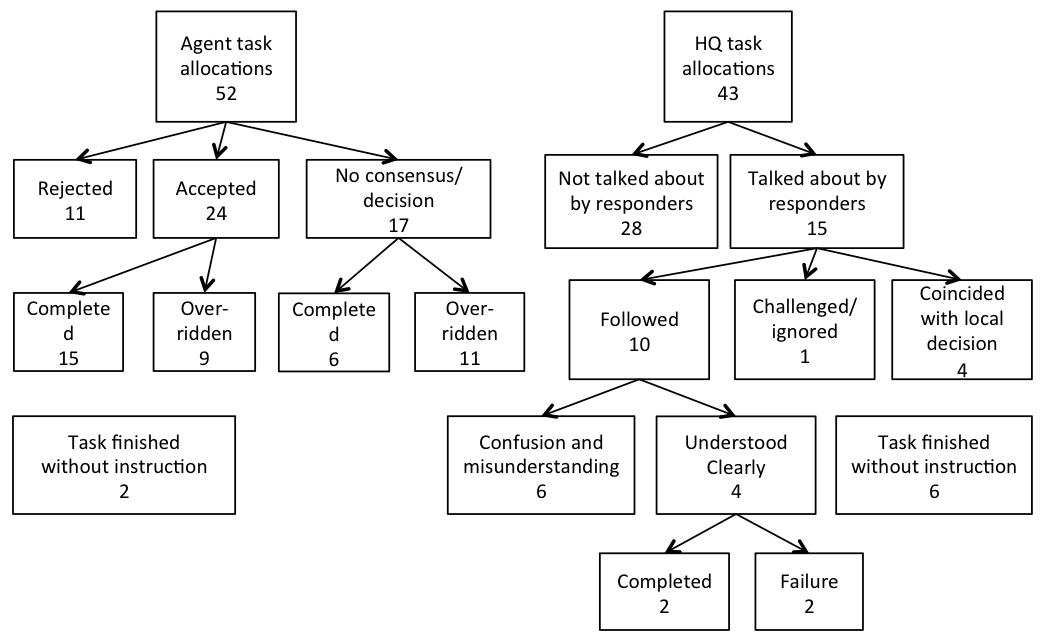
\includegraphics[width=\columnwidth]{message_handling.png}
\vspace{-5mm}
\caption{How task allocations were handled by FRs in the version with agent (left), and without agent (right). The `overridden' box denotes the number of times an `accepted' allocation in the non-agent case was not carried out to its full extent and, instead, another task was chosen by $H$ to be completed.}\label{fig:msgs}
\end{figure}


\begin{table}[ht]\small\centering
 \caption{Message classification.} \label{tab:msgs}
\begin{tabular}{c | c c | c c c c | c}
 & \multicolumn{2}{c|}{no agent} &  \multicolumn{4}{c|}{agent} & Total \\
 \hline
 Speech acts & \multicolumn{2}{c|}{Session A} & \multicolumn{2}{c}{Session B} & \multicolumn{2}{c|}{Session C} & \\
  & HQ & FR & HQ & FR & HQ & FR & \\
  \hline
  Directives & 89 & 0 & 34 & 2 & 34 & 0 & 159 \\
  Assertives & 33 & 6 & 26 & 16 & 24 & 16 & 121 \\
  \hline
  Total & 122 & 6 & 60 & 18 & 58 & 16 & 280 \\
\end{tabular}
\label{tab:assertives}
\end{table}


In contrast, when task allocation was handled by the agent (52 tasks allocated in two trials on average), FRs explicitly accepted 24 tasks,  of which they completed 15  successfully. Although there was either no response or no consensus between the FRs (in 17 tasks allocated), they still completed 6 of these tasks successfully. In total, 20 task allocations were withdrawn by the agent as a result of re-planning. 



%\paragraph{Rejecting task allocations}
In terms of task rejections, FRs rejected $PA$'s task allocation 11 times in the agent version. All of the rejections happened when the task allocation would have \emph{split existing teams}, or instructed FRs to team up with \emph{physically more distant FRs}. In most cases (9 out of 11), they triggered re-planning by rejection and \emph{adjusted the task allocation} to become consistent with the FR's current team. In the other two cases, the FRs rejected  the task allocation one more time before receiving the desired task allocation. For accepted instructions, the average distance between suggested teammates was 12 metres. For rejected instructions, the average was 86 metres.

The results above show that  the simple mechanism to get $PA$ to re-plan (i.e., reject/accept) was more successful (more tasks completed and less confusion) than the open-ended interactions between $H$ and the FRs (that were open to confusion).  Moreover, the fact that many of the rejections were due to the long distance to travel and teammate preference, implies that players chose to do the tasks they \emph{preferred}  rather than those deemed optimal by the agent. This indicates there may be an issue of trust in the agent, but also that it may be easier for a FR  to impose (through a reject) such preferences on an agent (and indirectly to other team members) rather than expressing this to $H$ or directly to teammates. 
% Role of HQ commander
It is also important to note that in the agent-assisted setting, $H$ frequently \emph{monitored} the allocation of tasks  returned by the agent (57 clicks on `show task' in UI FR status widget). Whereas 43 directives out of 68 in the non-agent session were task allocations, only 16 out of 68 were directly related to task allocations in the agent version. Out of these, $H$ directly reinforced the agent's instruction 6 times (e.g., ``SS and LT retrieve 09''), and complemented (i.e., added to or elaborated) $PA$'s task allocation 5 times (e.g., ``DP and SS, as soon as you can head to 20 before the radiation cloud gets there first''). $H$  did `override' $PA$'s instruction in 5 cases (as depicted by the `overridden' box).  

In the agent version, most of $H$'s directives (52 out of 68) and assertives (49 out of 51) focussed on providing situational awareness and  routing the FRs to avoid exposing them to radiation. For example, ``NK and JL approach drop off 6 by navigating via 10 and 09.'', or ``Radiation cloud is at the east of the National College''. 

These quantitative results point to the fact that H used PA as an advisor and in the non-agent case, H had to provide more information to FR on the ground. In fact,  during the debriefing session, the HQ operators in the non-agent case explicitly mentioned being overloaded by the number of variables under consideration when allocating tasks to FRs (e.g., providing situational awareness and allocating tasks) However, when supported by PA, the participants mentioned they trusted the agent to make the right decision and mainly spent time supervising its allocations or even improving the allocation in some cases. For example, in one instance, H explicitly advised FRs to go for a task that PA calculated would be covered by the radiation cloud before they could get there.  However, PA's estimates of FRs' running speed was obviously wrong in this case and the FRs were able to rescue the target. 


%\subsubsection{Summary and Guidelines}\label{sec:summary}
In summary, these results suggest three key observations with regard to  human-agent coordination in the trial: 
\begin{enumerate}
\item FRs performed better (rescued more targets)  and maintained higher health levels when supported by the agent.  These results echo those obtained under simulation (see Appendix \ref{sec:appendix2}) and  may reflect the better forward-planning capability of the planning agent compared to human FRs. 
 
\item Rejecting tasks was relatively frequently employed to trigger re-planning to obtain new task allocations aligned with FR preferences.  In each case, the planning agent was able to adapt to provide an alternative  that was acceptable to the FRs. Without this facility we believe the FRs would have chosen to ignore the plan. Task rejection seemed to be linked to changes to established teams, especially when members were relatively distant. Consequently, these kinds of allocations may need particularly support (e.g., explanation) or might be less preferentially selected by $PA$.

\item When task allocation was handled by $PA$, $H$ could focus on providing contingent and vital situational awareness to safely route first FRs around danger zones: thus demonstrating effective division of labour and complementary collaboration between humans and agents. We suggest that this effective division of labour contributes substantially to the observed performance increase of FRs when supported by the agent.
\end{enumerate}

Given the above observation we argue that a planning agent for team formation should not only model the uncertainty in player behaviours and in the environment, but that interactional challenges also need to be addressed  if such a technology is to be accepted in practice.  In the next section we elaborate on how our study results lead to new design guidelines for Human-Agent Collectives.

%\todo{--Gopal? Think this one's for you? (JF) -- the conclusions call for flexible autonomy, and this is somewhat supported by the algorithm and results. There are a few important limitations that the authors should discuss. For example, it is possible for responders to reject enough tasks tha the mission becomes infeasible. How would such a problem be addressed? The solution to such problems is beyond the scpoe of the paper but the relevant limitations of the algorithms are not.
%}




%\section{Real-world trial}
%We ran three sessions of AtomicOrchid with participants recruited from the local university to trial mixed-initiative coordination in a disaster response scenario. 
%
%\subsection{Participants and procedure}
%A total of 24 participants (7 of them were female) were recruited through posters and emails, and reimbursed with 15 pounds for 1.5-2 hours of study. The majority were students of the local university.
%
%The procedure consisted of 30 minutes of game play, and about 1 hour of pre-game briefing, consent forms and a short training session, and a post-game group discussion. 
%
%%Upon arrival in the HQ (set up in a meeting room at the local university), participants were briefed and asked to consent to participate. They were presented with a demographic questionnaire to record gender, occupation, experience of using smartphones and level of map navigation skills.
%
%At the end of the briefing in which mission objectives and rules were outlined, responder roles were randomly assigned to all participants (fire-fighter, medic, transporter, soldier). HQ was staffed by a different member of the research team in each session in order to mimick an experienced HQ whilst avoiding the same person running HQ every time. 
%
%Field responders were provided with a smartphone; HQ coordinators with a laptop. The team was given 5 minutes to discuss a common game strategy. 
%
%%(\textbf{Joel: where did the agent run ? --> Gopal, this should be covered in the previous section I think?})
%
%Field responders were then accompanied to the starting point within the designated game area, about 1 minute walk from headquarters. Once field responders were ready to start, HQ sent a `game start' message. After 30 minutes of game play the field responders returned to the HQ where a group interview was conducted, before participants were debriefed and dismissed.
%
%\subsection{Game sessions}
%We ran one session without the planner agent, and two sessions with the planner agent to be able to compare team performance in the two versions. We also ran a pilot study for each condition to fine tune game configuration. The 8 field responders in each session were randomly allocated a responder so that the whole team had two of each of the four kinds of responder roles. The terrain of the 400x400metres game area includes grassland, a lake, buildings, roads, and footpaths and lawns. There were two drop off zones and 16 targets in each session. There were four targets for each of the four target types. The target locations, pattern of cloud movement and expansion were kept constant for all game sessions. The pilot study showed that this was a challenging, yet not too overwhelming configuration of game area size, and number of targets to collect in a 30 min game session. 
%
%\subsection{Data collection and analysis}
%We developed a log file replay tool to triangulate video recordings of game action with the time stamped system logs that contain a complete record of the game play, including responders' GPS location, their health status and radioactive exposure, messages, cloud location, locations of target objects and task status.
%
%%Video recordings of field action were catalogued to identify sequences (episodes) of interest (cf. Heath et al., 2010). Key decision points in teaming and task allocation served to index the episodes. Interesting distinct units of interaction were transcribed and triangulated with log files of relevant game activity for deeper analysis. Due to space constraints we can only  present one fragment in this paper to illustrate how human-agent collaboration typically unfolded (TODO).
%
%In this paper we focus on how both agent task allocations and remote messages are used as a coordination resource. We use speech-act theory (Searle, 1975) to classify messages sent between and among responders and HQ. We focus on the most relevant types of acts in this paper (which are also the most frequently used in AtomicOrchid):
%
%\begin{itemize}
%\item Assertives: \textit{speech acts that commit a speaker to the truth of the expressed proposition}; these were a common category as they include messages that contain situational information.
%\item Directives: \textit{speech acts that are meant to cause the hearer to take a particular action}, e.g. requests, commands and advice, including task and team allocation messages. 
%\end{itemize}
%
%\subsection{Results}
%Overall, 8 targets were rescued in the non-agent condition (Session A), and respectively 12 targets (Session B), and 11 targets (Session C) were rescued in the agent condition. Teams (re-)formed six times in session A, four times in session B and nine times  in session C. Average player health after the game was 40/100 in Session B, and 81 for the agent-assisted sessions (B:80, C: 82). One responder `died' in Session A.  
%
%The agent dynamically re-planned 14 times in session B, and 18 times in session C. Most of the times, this was triggered when a target was dropped off in the safe zone (24 times), some times this was triggered by a player rejecting the agent's task allocation (8 times). 
%
%Table \ref{tab:msgs} shows the directives (mainly related to task allocation and execution) and assertives (mainly related to situational awareness) sent in the sessions. The next sections draw on how these messages were handled to give a sense of mixed-initiative coordination in the game sessions.
%
%\begin{table}\footnotesize
%\begin{tabular}{c | c c | c c c c | c}
% & \multicolumn{2}{c|}{no agent} &  \multicolumn{4}{c|}{agent} & Total \\
% \hline
% Speech acts & \multicolumn{2}{c|}{Session A} & \multicolumn{2}{c}{Session B} & \multicolumn{2}{c|}{Session C} & \\
%  & HQ & FR & HQ & FR & HQ & FR & \\
%  \hline
%  Directives & 89 & 0 & 34 & 2 & 34 & 0 & 159 \\
%  Assertives & 33 & 6 & 26 & 16 & 24 & 16 & 121 \\
%  \hline
%  Total & 122 & 6 & 60 & 18 & 58 & 16 & 280 \\
%\end{tabular}
% \label{tab:msgs}
% \caption{Message classification.}
%\end{table}
%
%
%\subsubsection{Handling task allocations}
%Fig. \ref{fig:msgs} shows how field responders handled task allocations in the agent and in the non-agent condition. In the non-agent condition, HQ sent 43 task allocation directives. Out of these, the recipient field responders addressed only 15 messages (bringing them up in conversation). Out of these 15, responders chose to ignore the instructions only once. The responder ignored the instruction because they were engaged in another task and did not want to abandon it. A further 4 HQ instructions were consistent with a decision to rescue a certain target that has already been made locally by the responders. In 10 cases field responders chose to follow the instructions. Although players were willing to follow HQ's instructions, they failed to correctly follow the instructions due to confusion and misunderstanding in the communication. In fact, only 2 instances of directives from the HQ led to task completion.The field responders accomplished task allocation of the other 6 saved targets locally without being instructed by HQ.
%
%On the other hand, when task allocation was handled by the agent, responders accepted 24 tasks, out of which they completed 15 tasks successfully. Even if there was no response or consensus between the responders (in 17 cases), still six out of 17 tasks were completed successfully. In total, 20 task allocations were overridden by a the agent with a new task allocation. 
%
%\begin{figure}[htbp]
%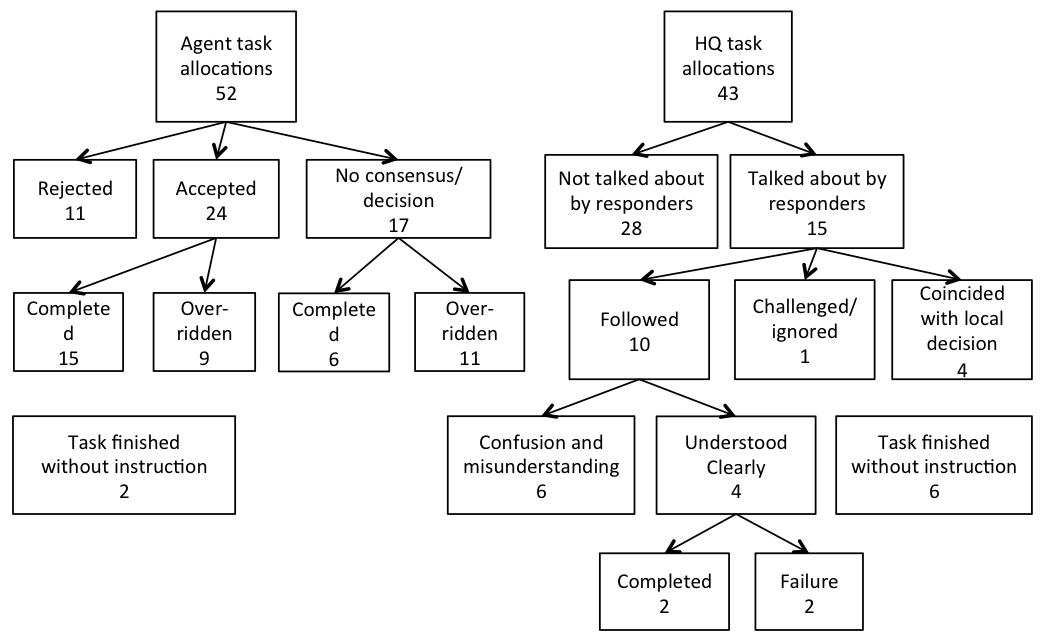
\includegraphics[width=\columnwidth]{message_handling.png}
%\label{fig:msgs}
%\caption{How task allocations were handled by field responders in the agent version (left) and in the non-agent version (right).}
%\end{figure}
%
%\paragraph{Rejecting task allocations}
%
%Field responders rejected the agent's task allocation 11 times in the agent version. All of the rejections happened when the task allocation would have split existing teams, or instructed responders to team up with physically more distant responders. In most cases (9 out of 11), the rejection triggered re-planning and adjusted the task allocation to become consistent with the responder's current team. In the other 2 cases, rejected the task allocation one more time to receive the desired task allocation. 
%
%Overall, players were more likely to reject plan if their proposed teammates were far away from them. For accepted instructions, the average distance between suggested teammates was 12 metres. For rejected instructions, the average distance between suggested teammates was 86 metres.
%
%\subsubsection{The role of HQ}
%The role of HQ changed in that in the non-agent version HQ was responsible for handling task allocations, whereas task allocation was handled by the agent in the other version. HQ frequently monitored the agent's task allocation in the two agent-supported sessions (57 clicks on `show task' in UI responder status widget). Whereas 43 directives in the non-agent session were task allocations, only 16 out of 68 directives were directly related to task allocations in the agent version. Out of these, HQ reinforced the agent instruction 6 times (e.g., ``SS and LT retrieve 09''), and complemented the agent's task allocation 5 times (``DP and SS, as soon as you can head to 20 before the radiation cloud gets there first''). HQ did `override' the agent instruction in 5 cases.  
%
%In the agent version, the majority of HQ's directives (52 out of 68) and assertives (49 out of 51) focussed on providing situational awareness and safely routing the responders to avoid exposing them to radiation. For example, ``Nk and JL approach drop off 6 by navigating via 10 and 09.'', or ``Radiation cloud is at the east of the National College''. 
%
%\subsubsection{Summary}
%The results suggest three key observations with regard to mixed-initiative coordination in the trial:
%
%\begin{itemize}
%\item Field responders performed better (rescued more targets), and maintained higher health levels when supported by the agent.
%\item Rejecting tasks was a frequently employed method to to trigger re-planning to obtain new task allocations aligned with responder preferences.
%\item When task allocation was handled by the agent, the human HQ could focus on providing vital situational awareness to safely route field responders around danger zones; thus demonstrating division of labour and complementary collaboration between human and agent.
%\end{itemize}
%
% 
%%Joel and Wenchao
%%\begin{enumerate}
%%\item Explain setup of experiment - area of interest + setup of tasks
%%\item Explain evaluation = quantitative and qualitative.
%%\end{enumerate}
%%\paragraph{Metrics}
%%\begin{itemize}
%%\item{Comparisons between with/without agent versions for the below:}
%%\item{Performance of FR: number of tasks completed, time on task?, number of messages sent, number of teams formed and disbanded, time on team, acknowledgements of tasks}
%%\item{Messages: classification}
%%\item{Health}
%%\item{Distance travelled}
%%\item{HQ: number of agent monitoring actions (clicks), number of 'supporting'/related messages (e.g., enforcement, contradictions/overriding)}
%%\item{Agent performance: number of instructions, number of replanning steps, replanning robustness (diversion of task allocation compared to previous step)}
%%\item{Following instructions ('obedience'): number of instructions followed vs. not followed (incl. number of HQ interventions/overriding agent allocation), instruction handling diagram}
%%\item
%%\end{itemize}
